\documentclass[12pt]{article}

\usepackage[13643]{easymcm}  % Team control number
\usepackage{longtable}
\usepackage{booktabs}

\problem{A}  % Problem number

\title{Paper Name}  % Title

\begin{document}

\begin{abstract}

	Some random text
	
\end{abstract}

\maketitle
\tableofcontents

\section{Introduction}

	\subsection{Problem Background}
		
		
		
	\subsection{Problem Restatement}
	
		some random text

\section{Dandelion Spread Model}

	\subsection{Assumptions and Justifications}
	
		\begin{enumerate}
			
			\item The dandelion is located at the midpoint of an edge of a square field of dimensions 100m$\times$100m (1 hectare).  When seeds are blown out of the field, they are neglected.
			\vspace{-0.125in}
			\begin{description}
				\item[Justification:] The problem states that the dandelion is adjacent to the field.  Thus, we consider the dandelion to be located on the edge of the field.  Furthermore, we limit our consideration within the field.  Seeds that land outside the field are considered to be negligible
			\end{description}
			
			\item Assumption 4
			\vspace{-0.125in}
			\begin{description}
				\item[Justification:] The frea
			\end{description}
			
			\item Assumption 4
			\vspace{-0.125in}
			\begin{description}
				\item[Justification:] The frea
			\end{description}
			
			\item Assumption 4
			\vspace{-0.125in}
			\begin{description}
				\item[Justification:] The frea
			\end{description}
			
		\end{enumerate}
	
	\subsection{Environmental Factors}
	
		\begin{figure}
			\centering
			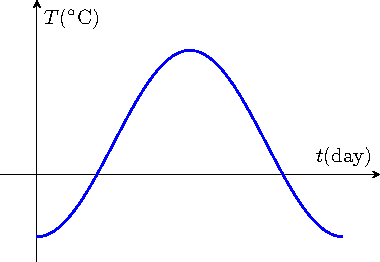
\includegraphics{fig-temperature_curve.pdf}
			\caption{Temperature curve}
			\label{fig:temp}
		\end{figure}
	
	\subsection{Dandelion Life Cycle}
	
		\begin{figure}
			\centering
			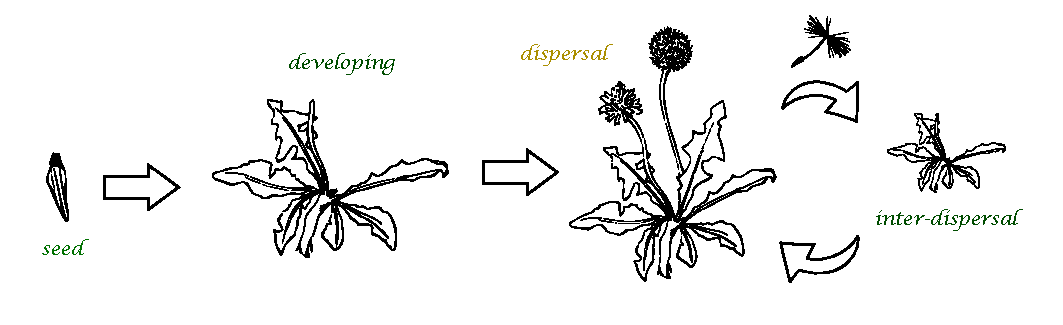
\includegraphics {life_cycle.pdf}
			\caption{Dandelion life cycle}
			\label{fig:lifeCycle}
		\end{figure}

	\subsection{Dandelion Life Cycle}

	\begin{figure}
		\centering
		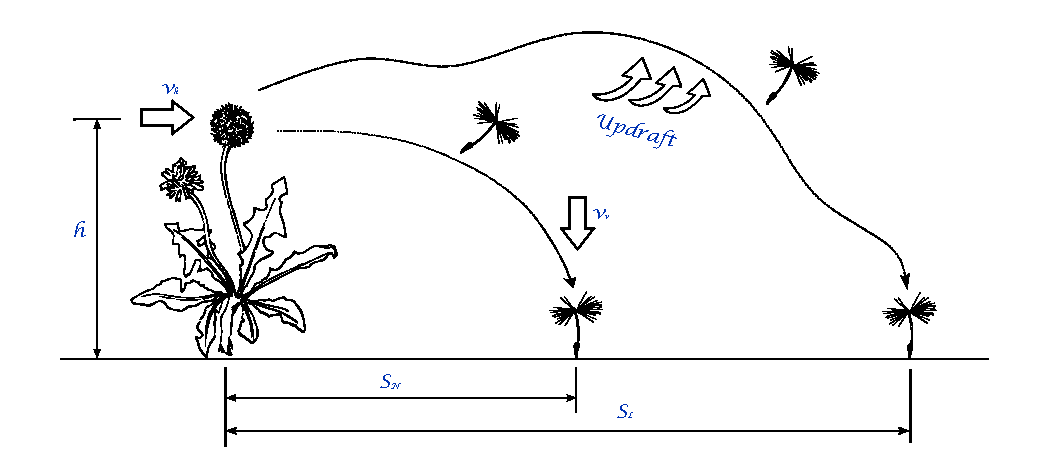
\includegraphics {wind_mode.pdf}
		\caption{Dandelion dispersal distance}
		\label{fig:dispersal}
	\end{figure}
	
	\subsection{Dispersal Distance}
		
		\begin{figure}
			\centering
			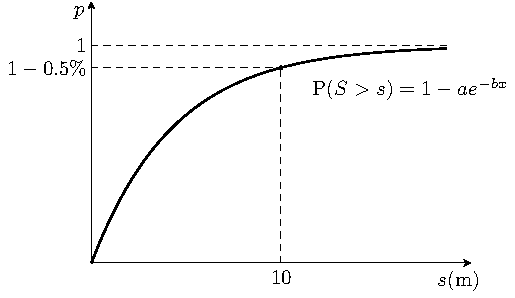
\includegraphics{fig-wind_curve.pdf}
			\caption{Cumulative distribution function of long-distance dispersal}
			\label{fig:longDistance}
		\end{figure}
		
	\subsection{Algorithm}
	
	\subsection{Dandelion Spread Results}
	
		\subsubsection{Results}
		
			text
			
			\begin{figure}
				\centering
				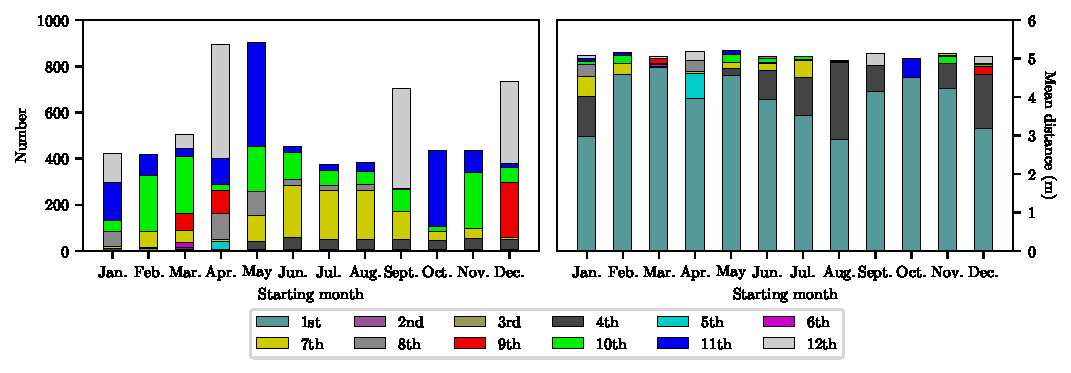
\includegraphics{start_month-number.pdf}
				\caption{Number and mean distance of dandelions in Florida when simulation starts at different times}
				\label{fig:start}
			\end{figure}
			
			\begin{figure}
				\centering
				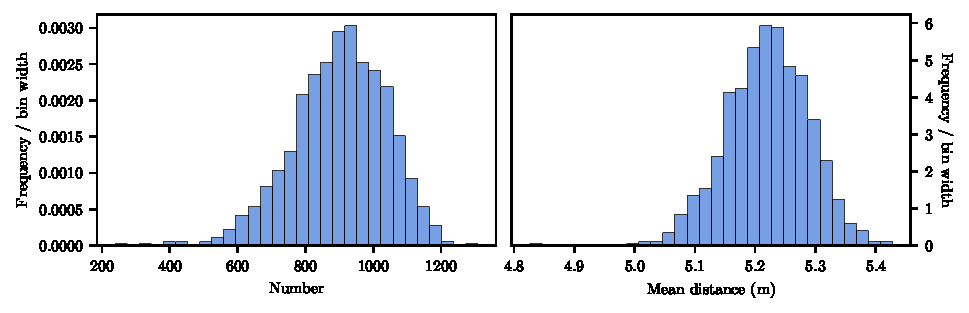
\includegraphics{number-frequency.pdf}
				\caption{Frequency distribution of number and mean distance of dandelions in Florida}
				\label{fig:freqDand}
			\end{figure}
			
			
			\begin{figure}
				\centering
				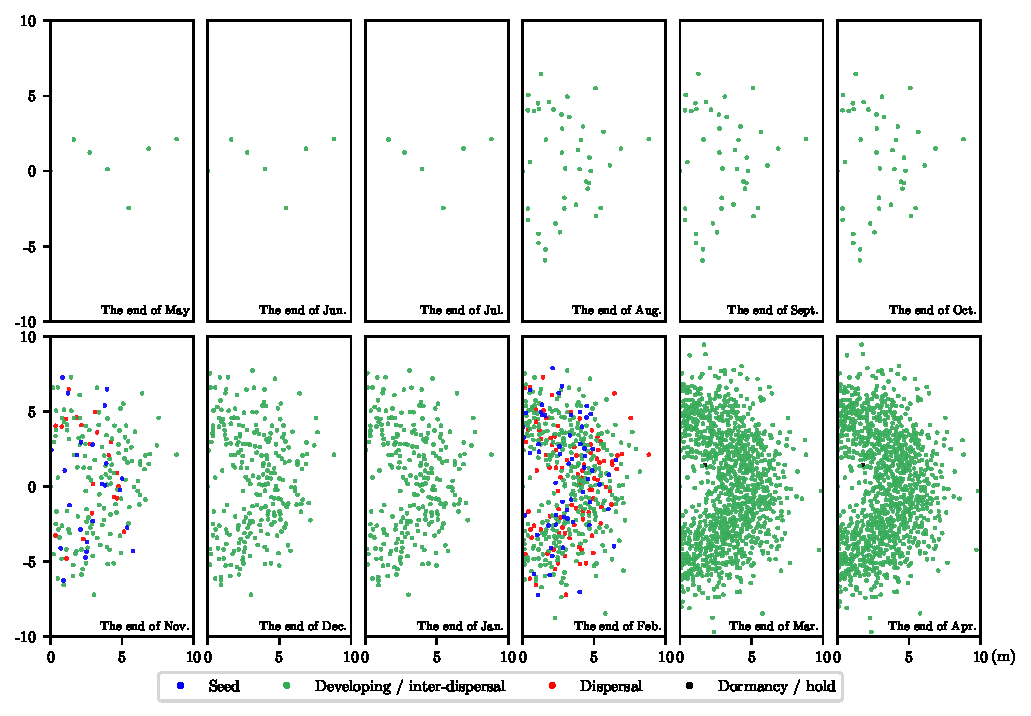
\includegraphics{spread_course-time.pdf}
				\caption{The spread of dandelion during a 12-month period in the District of Columbia}
				\label{fig:spreadDC}
			\end{figure}
			
			Lorem ipsum dolor sit amet Lorem ipsum dolor sit amet Lorem ipsum dolor sit amet Lorem ipsum dolor sit amet Lorem ipsum dolor sit amet Lorem ipsum dolor sit amet Lorem ipsum dolor sit amet Lorem ipsum dolor sit amet Lorem ipsum dolor sit amet Lorem ipsum dolor sit amet Lorem ipsum dolor sit amet Lorem ipsum dolor sit amet Lorem ipsum dolor sit amet Lorem ipsum dolor sit amet Lorem ipsum dolor sit amet Lorem ipsum dolor sit amet Lorem ipsum dolor sit amet Lorem ipsum dolor sit amet Lorem ipsum dolor sit amet Lorem ipsum dolor sit amet Lorem ipsum dolor sit amet Lorem ipsum dolor sit amet Lorem ipsum dolor sit amet Lorem ipsum dolor sit amet Lorem ipsum dolor sit amet Lorem ipsum dolor sit amet Lorem ipsum dolor sit amet Lorem ipsum dolor sit amet Lorem ipsum dolor sit amet Lorem ipsum dolor sit amet Lorem ipsum dolor sit amet Lorem ipsum dolor sit amet Lorem ipsum dolor sit amet Lorem ipsum dolor sit amet Lorem ipsum dolor sit amet Lorem ipsum dolor sit amet Lorem ipsum dolor sit amet Lorem ipsum dolor sit amet Lorem ipsum dolor sit amet Lorem ipsum dolor sit amet Lorem ipsum dolor sit amet Lorem ipsum dolor sit amet Lorem ipsum dolor sit amet Lorem ipsum dolor sit amet Lorem ipsum dolor sit amet Lorem ipsum dolor sit amet Lorem ipsum dolor sit amet Lorem ipsum dolor sit amet Lorem ipsum dolor sit amet Lorem ipsum dolor sit amet Lorem ipsum dolor sit amet Lorem ipsum dolor sit amet Lorem ipsum dolor sit amet Lorem ipsum dolor sit amet Lorem ipsum dolor sit amet Lorem ipsum dolor sit amet Lorem ipsum dolor sit amet Lorem ipsum dolor sit amet Lorem ipsum dolor sit amet Lorem ipsum dolor sit amet 
			
			\begin{figure}
				\centering
				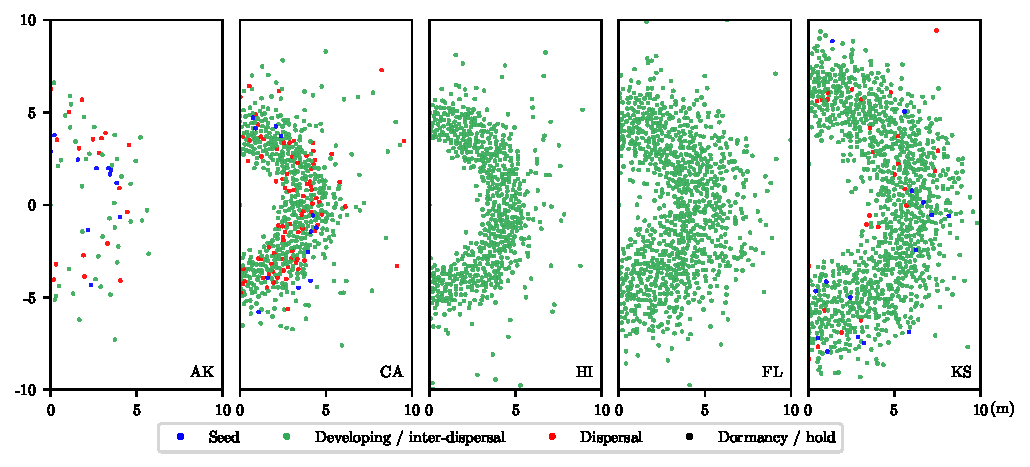
\includegraphics{spread_course-location_non_DC.pdf}
				\caption{The spread of dandelions at the end of 12 months at different locations}
				\label{fig:scatter5loc}
			\end{figure}
			
			Lorem ipsum dolor sit amet Lorem ipsum dolor sit amet Lorem ipsum dolor sit amet Lorem ipsum dolor sit amet Lorem ipsum dolor sit amet Lorem ipsum dolor sit amet Lorem ipsum dolor sit amet Lorem ipsum dolor sit amet Lorem ipsum dolor sit amet Lorem ipsum dolor sit amet Lorem ipsum dolor sit amet Lorem ipsum dolor sit amet Lorem ipsum dolor sit amet Lorem ipsum dolor sit amet Lorem ipsum dolor sit amet
			
					
			\begin{figure}
				\centering
				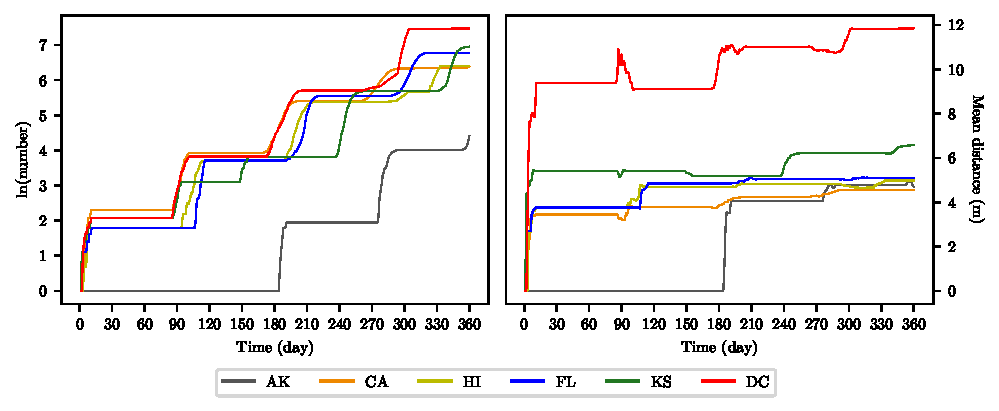
\includegraphics{number_mean_distance-time.pdf}
				\caption{Number and mean distance of dandelions plotted against time}
				\label{fig:time}
			\end{figure}
		
		\subsubsection{Sensitivity Analysis}
		
			\begin{figure}
				\centering
				\begin{minipage}{0.04\textwidth}\end{minipage}
				\begin{minipage}{0.46\textwidth}
					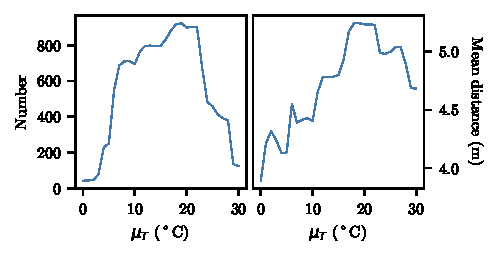
\includegraphics{sa_MuT.pdf}
				\end{minipage}
				\begin{minipage}{0.46\textwidth}
					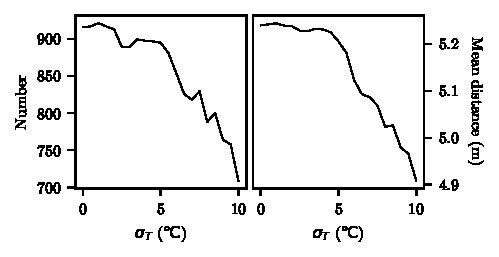
\includegraphics{sa_StdT.pdf}
				\end{minipage}
				\begin{minipage}{0.04\textwidth}\end{minipage}
				
				\begin{minipage}{0.04\textwidth}\end{minipage}
				\begin{minipage}{0.46\textwidth}
					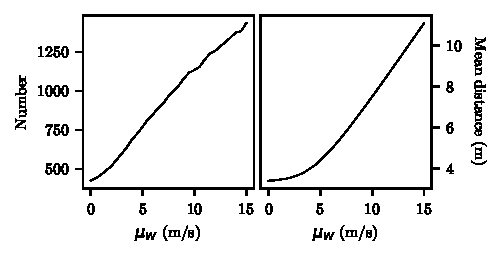
\includegraphics{sa_MuW.pdf}
				\end{minipage}
				\begin{minipage}{0.46\textwidth}
					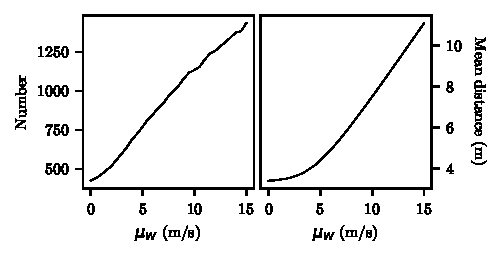
\includegraphics{sa_MuW.pdf}
				\end{minipage}
				\begin{minipage}{0.04\textwidth}\end{minipage}
				
				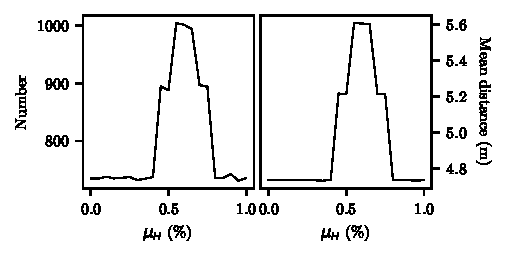
\includegraphics{sa_Hum.pdf}
				\caption{Sensitivity analysis}
				\label{fig:sa}
			\end{figure}
			
		\subsubsection{Strengths and Weaknesses}
		
	\subsection{Dandelion Spread Fitting Model}
		
		\subsubsection{Data}
		
		\subsubsection{Algorithm}
		
		\subsubsection{Results}
		
		\subsubsection{Sensitivity Analysis}
		
		\subsubsection{Strengths and Weaknesses}
	
			some random text
		
\section{Plant Impact Factor Model}

	\subsection{Assumptions and Justifications}
	
	\subsection{Model Description}

		hello
		
		{
			\fontsize{10}{13}\selectfont
			{
			\begin{longtable}{p{0.2in}p{1.5in}p{4.3in}}
			
				\toprule
				\multicolumn{1}{c}{\textbf{Symbol}} 
					& \multicolumn{1}{c}{\textbf{Aspect}}
					& \multicolumn{1}{c}{\textbf{$a_i$, $b_i$ and $c_i$ Evaluation}} \\
			
				\toprule
				\multicolumn{3}{l}{Category $A$ - Plant Characteristics}\\
				\midrule
				
				$A_1$ & Duration & $a_1=0.5$ (Annual), $0.75$ (Biennial), $1$ (Perennial)\\
				$A_2$ & Growing Habit & $a_2=0$ (Tree), $0.25$ (Shrub), $0.5$ (Vine), $0.75$ (Graminoid), $1$ (Forb/herb)\\ 
				$A_3$ & Growth Rate & The growth rate after successful establishment\\
					&& $a_3=0.5$ (Slow), $0.75$ (Moderate), $1$ (Rapid)\\
				$A_4$ & Lifespan & $a_4=0.25$ (when $a_1=0.5$ or $0.75$), $0.5$ (Short), $0.75$ (Moderate), $1$ (Long) \\
				$A_5$ & Fertility Requirement & Relative level of nutrition (N, P, K) required for normal growth and development.\\
					 && $a_5=0.5$ (Low), $0.75$ (Medium), $1$ (High)\\
				$A_6$ & Fruit/Seed Abundance & The amount of seed produced.\\
					&& $a_6=0.25$ (None), $0.5$ (Low), $0.75$ (Medium), $1$ (High)\\
				$A_7$ & Propagated Methods & The propagetion methods number, $n_7$. The methods can be Propagated by Bare Root, by Bulb, by Container, by Corm, by Cuttings, by Seed, by Sod, by Sprigs, or by Tubers. \\
					&& $a_7=0.25$ ($n_7=1$), $0.5$ ($n_7=2$), $0.75$ ($n_7=3$), $1$ ($n_7\geq4$)\\
				$A_8$ & Seed Spread Rate & The capability of the plant to spread through its seed production.\\
					&& $a_8=0.25$ (None), $0.5$ (Slow), $0.75$ (Moderate), $1$ (Rapid)\\
				$A_9$ & Seedling Vigor & The expected seedling survival percentage of the plant\\
					&& $a_9=0.5$ (Low), $0.75$ (Medium), $1$ (High)\\
				
				\midrule
				\multicolumn{3}{l}{Category $B$ - Human and Environment}  \\
				\midrule
				
				$B_1$ & Toxicity & The relative toxicity of the plant to either humans or livestock.\\
					&& $b_1=0$ (None), $0.5$ (Slight), $0.75$ (Moderate), $1$ (Severe)\\
				$B_2$ & Product & The level of the plant known to be suitable for multiple types of products.\\
					&& $b_2=0$ (Copiousness), $0.25$ (Many), $0.5$ (Some), $0.75$ (few), $1$ (None)\\
				$B_3$ & Palatable Animal & The relative palatability of this plant to browsing animals or to grazing animals.\\
					&& $b_3=0$ (High), $0.5$ (Moderate), $0.75$ (Low), $1$ (None)\\
				$B_4$ & Palatable Human & The plant produce berries, nuts, seeds, or fruits are palatable to humans. \\
					&& $b_4=0.5$ (Yes), $1$ (No)\\
				$B_5$ & Commercial Availability & The plant propagules are in the commercial marketplace \\
					&& $b_5=0.5$ (Yes), $1$ (No)\\
			
				\midrule
				\multicolumn{3}{l}{Category $C$ - Location}  \\
				\midrule
				
				$C_1$ & Soil Adaption & The soil is suitable for the plane\\
					&& $c_1=0.5$ (Yes), $1$ (No)\\
				$C_2$ & Temperature Adaption & The temperature is suitable for the plane\\
					&& $c_2=0.5$ (Yes), $1$ (No)\\
				$C_3$ & Humid Adaption & The humid is suitable for the plane\\
					&& $c_3=0.5$ (Yes), $1$ (No)\\
				$C_4$ & Population Density & The level of population density.\\
					&& $c_4=0.5$ (High), $1$ (Medium), $1$ (Low)\\
			
				\bottomrule
			
			\end{longtable}
			}
		}
		
		{
			\fontsize{10}{18}\selectfont
			{
				\begin{longtable}{c|ccccccccc|ccccc||cccc}
					\toprule
					&$A_1$&$A_2$&$A_3$&$A_4$&$A_5$&$A_6$&$A_7$&$A_8$&$A_9$&$B_1$&$B_2$&$B_3$&$B_4$&$B_5$&$C_1$&$C_2$&$C_3$&$C_4$\\
					\toprule
					$A_1$&$1$&$1/3$&$1/7$&$1/3$&$1$&$1/7$&$1/4$&$1/7$&$1/5$&$1/9$&$1/5$&$1/3$&$1/4$&$1/4$&$1/5$&$1/5$&$1/5$&$1/3$\\
					$A_2$&$3$&$1$&$1/5$&$1$&$3$&$1/5$&$1/2$&$1/5$&$1/3$&$1/7$&$1/3$&$1$&$1/2$&$1/2$&$1/3$&$1/3$&$1/3$&$1$\\
					$A_3$&$7$&$5$&$1$&$5$&$7$&$1$&$4$&$1$&$3$&$1/3$&$3$&$5$&$4$&$4$&$3$&$3$&$3$&$5$\\
					$A_4$&$3$&$1$&$1/5$&$1$&$3$&$1/5$&$1/2$&$1/5$&$1/3$&$1/7$&$1/3$&$1$&$1/2$&$1/2$&$1/3$&$1/3$&$1/3$&$1$\\
					$A_5$&$1$&$1/3$&$1/7$&$1/3$&$1$&$1/7$&$1/4$&$1/7$&$1/5$&$1/9$&$1/5$&$1/3$&$1/4$&$1/4$&$1/5$&$1/5$&$1/5$&$1/3$\\
					$A_6$&$7$&$5$&$1$&$5$&$7$&$1$&$4$&$1$&$3$&$1/3$&$3$&$5$&$4$&$4$&$3$&$3$&$3$&$5$\\
					$A_7$&$4$&$2$&$1/4$&$2$&$4$&$1/4$&$1$&$1/4$&$1/2$&$1/4$&$1/2$&$2$&$1$&$1$&$1/2$&$1/2$&$1/2$&$2$\\
					$A_8$&$7$&$5$&$1$&$5$&$7$&$1$&$4$&$1$&$3$&$1/3$&$3$&$5$&$4$&$4$&$3$&$3$&$3$&$5$\\
					$A_9$&$5$&$3$&$1/3$&$3$&$5$&$1/3$&$2$&$1/3$&$1$&$1/5$&$1$&$3$&$2$&$2$&$1$&$1$&$1$&$3$\\
					\midrule
					$B_1$&$9$&$7$&$3$&$7$&$7$&$3$&$4$&$3$&$5$&$1$&$5$&$7$&$4$&$4$&$5$&$5$&$5$&$7$\\
					$B_2$&$5$&$3$&$1/3$&$3$&$5$&$1/3$&$2$&$1/3$&$1$&$1/5$&$1$&$3$&$2$&$2$&$1$&$1$&$1$&$3$\\
					$B_3$&$3$&$1$&$1/5$&$1$&$3$&$1/5$&$1/2$&$1/5$&$1/3$&$1/7$&$1/3$&$1$&$1/2$&$1/2$&$1/3$&$1/3$&$1/3$&$1$\\
					$B_4$&$4$&$2$&$1/4$&$2$&$4$&$1/4$&$1$&$1/4$&$1/2$&$1/4$&$1/2$&$2$&$1$&$1$&$1/2$&$1/2$&$1/2$&$2$\\
					$B_5$&$4$&$2$&$1/4$&$2$&$4$&$1/4$&$1$&$1/4$&$1/2$&$1/4$&$1/2$&$2$&$1$&$1$&$1/2$&$1/2$&$1/2$&$2$\\
					\midrule
					\midrule
					$C_1$&$5$&$3$&$1/3$&$3$&$5$&$1/3$&$2$&$1/3$&$1$&$1/5$&$1$&$3$&$2$&$2$&$1$&$1$&$1$&$3$\\
					$C_2$&$5$&$3$&$1/3$&$3$&$5$&$1/3$&$2$&$1/3$&$1$&$1/5$&$1$&$3$&$2$&$2$&$1$&$1$&$1$&$3$\\
					$C_3$&$5$&$3$&$1/3$&$3$&$5$&$1/3$&$2$&$1/3$&$1$&$1/5$&$1$&$3$&$2$&$2$&$1$&$1$&$1$&$3$\\
					$C_4$&$3$&$1$&$1/5$&$1$&$3$&$1/5$&$1/2$&$1/5$&$1/3$&$1/7$&$1/3$&$1$&$1/2$&$1/2$&$1/3$&$1/3$&$1/3$&$1$\\
					\bottomrule
				\end{longtable}
			}
		}	
	
		hello!!! \\

	\subsection{Sensitivity Analysis}
	
		\begin{figure}
			\centering
			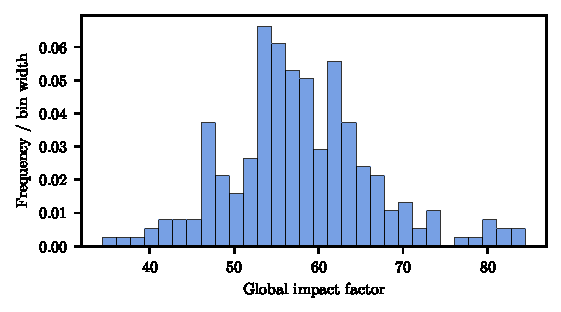
\includegraphics{IF-frequency.pdf}
			\caption{Frequency distribution of global impact factor}
			\label{fig:freqIF}
		\end{figure}
	
		\begin{figure}
			\centering
			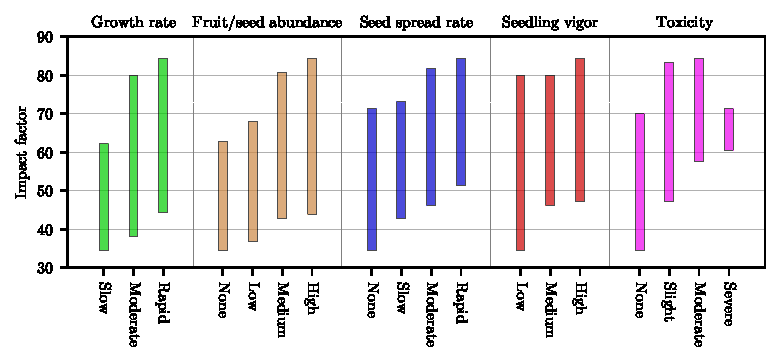
\includegraphics{categories-IF.pdf}
			\caption{What caption should this figure have?}
			\label{fig:IFfactors}
		\end{figure}
		
		\begin{figure}
			\centering
			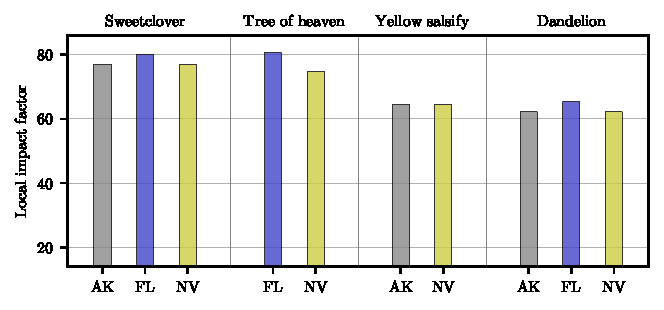
\includegraphics{IF_local-loc.pdf}
			\caption{What caption should this figure have?}
			\label{fig:IFLocal}
		\end{figure}
		
	\subsection{Strengths and Weaknesses}

		some random text
	
\section*{We Share the Earth}
\addcontentsline{toc}{section}{We Share the Earth}



\newrefcontext
\printbibliography

\end{document}
